%!TEX root = ../09-Photoelectric-Effect.tex
\chapter{Photoelectric Effect}


\section{Open Circuit Voltage}%3.1


\section{Stopping Voltage}%3.2 and 3.5


\section{Photocurrent}%3.3 and 3.4

The current flowing through the photoelectric cell is measured while the voltage across it's terminals is held at constant levels ranging from \SIrange{-3}{6}{\volt}.

A schematic of the setup is shown in \autoref{sch:photocurrent}.
A shunt resistor of $R_\text{shunt} = \SI{100}{\mega\ohm}$ is used, the output voltage is buffered by the electrometer to minimize the additional load.
The voltage $U_\text{g}$ is generated by a potentiometer connected across a \SI{9}{\volt} battery, it is read from a panel meter.

The actual stopping potential is $U_\text{s} = U_\text{g} - U_\text{out}$.

\begin{figure}[tbp]
	\centering
	\includegraphics[width=.4\textwidth]{img/photocurrent.pdf}
	\caption[Setup for measuring Photocurrent]{\textbf{Setup for measuring Photocurrent}}
	\label{sch:photocurrent}
\end{figure}

\begin{figure}[tbp]
	\centering
	\includegraphics[width=.8\textwidth]{data/plots/photocurrent.pdf}
	\caption[Photocurrent versus Stopping Potential]{\textbf{Photocurrent versus Stopping Potential}}
	\label{plt:photocurrent}
\end{figure}
